
%(BEGIN_QUESTION)
% Copyright 2006, Tony R. Kuphaldt, released under the Creative Commons Attribution License (v 1.0)
% This means you may do almost anything with this work of mine, so long as you give me proper credit

What will be wrong with this measurement system if we connect a linear-scale indicator (an electrical meter movement responding to the transmitter's current signal) to the transmitter's output, and try to measure fluid flow along this scale?  Assume the transmitter has been properly calibrated to output full current (typically 20 mA) at full flow through the orifice plate.

$$\includegraphics[width=10cm]{i00483x01.eps}$$

Hint: what will the meter indicate when the actual flow rate is at 0\%, 50\%, and 100\%?

\underbar{file i00483}
%(END_QUESTION)





%(BEGIN_ANSWER)

At 0\% flow and 100\% flow rates, the meter will indicate accurately.  It will be very much in error at any point in between.  At 50\% true flow rate, for example, the meter will only indicate 25\%, since the differential pressure drop generated by the orifice plate will only be that much at the half-flow rate.

\vskip 10pt

Follow-up question: identify a way we may correct this system so that all the points along the indicator's scale accurately reflect flow rate through the orifice.

%(END_ANSWER)





%(BEGIN_NOTES)

Electrical meter movements are usually linear devices.  Differential pressure transmitters are usually linear devices.  Orifice plates are nonlinear in the pressure drop they generate for various flow rates.  Since the differential pressure drop across the orifice plate is nonlinear, the linear differential pressure transmitter will simply repeat this nonlinearity to the meter movement, which repeats the nonlinearity to the scale.

The accuracy -- and the linearity -- of any metering system depends on each and every link in the chain of communication.  In order to make the system register linearly from orifice plate to meter, we must add a complementary nonlinearity to the system designed to correct for the nonlinearities of the orifice plate.  One way to do this is make the meter scale nonlinear.  Another way to do this is add a signal converter to the loop performing the square root math function, to ``undo'' the square characteristic of the orifice plate.

%INDEX% Measurement, flow: orifice plate

%(END_NOTES)


